\documentclass{scrartcl}
\usepackage{pgfplots}
\pgfplotsset{compat=1.8}
\usepgfplotslibrary{statistics}
\usepackage[ngerman]{babel}
\usepackage[fleqn]{amsmath}
\usepackage{amssymb}
\usepackage{bbm}
\usepackage{graphicx}
\usepackage{setspace}
\usepackage{listings}
\usepackage{pdfpages}
\usepackage{algorithm} 
\usepackage{algorithmic}
\usepackage{hyperref}
\usepackage{makecell}
\usepackage{longtable}
\usetikzlibrary{trees}
\newcommand{\bbN}{\mathbbm{N}}
\newcommand{\bbR}{\mathbbm{R}}
\newcommand{\bbZ}{\mathbbm{Z}}
\newcommand{\bbI}{\mathbbm{I}}
\usepackage{tikz}
\usetikzlibrary{plotmarks}
\usepackage[left=2cm,right=2cm,top=1.5cm,bottom=2cm]{geometry} % Seiteneinrichtung
\pgfplotsset{compat=1.8}

\begin{document}
\title{Architekturbeschreibung: Mikrokontroller für FPGA-Board}
\subtitle{Gruppe 2}
\author{Jannik Graef 3392032 st161399@stud.uni-stuttgart.de \and
 Tobias Weinschenk 3404690 st161650@stud.uni-stuttgart.de \and
 Jochen Benzenhöfer 3456431 st166313@stud.uni-stuttgart.de \and
 Alexander Bunz 3456583 st166212@stud.uni-stuttgart.de \and
 Omar Al Kadri 3456978 st166418@stud.uni-stuttgart.de \and
 Simon Naß 3460883 st166318@stud.uni-stuttgart.de \and
 Jonas Unterweger 3464025 st167417@stud.uni-stuttgart.de}
\maketitle


\section{Blockdiagram}
    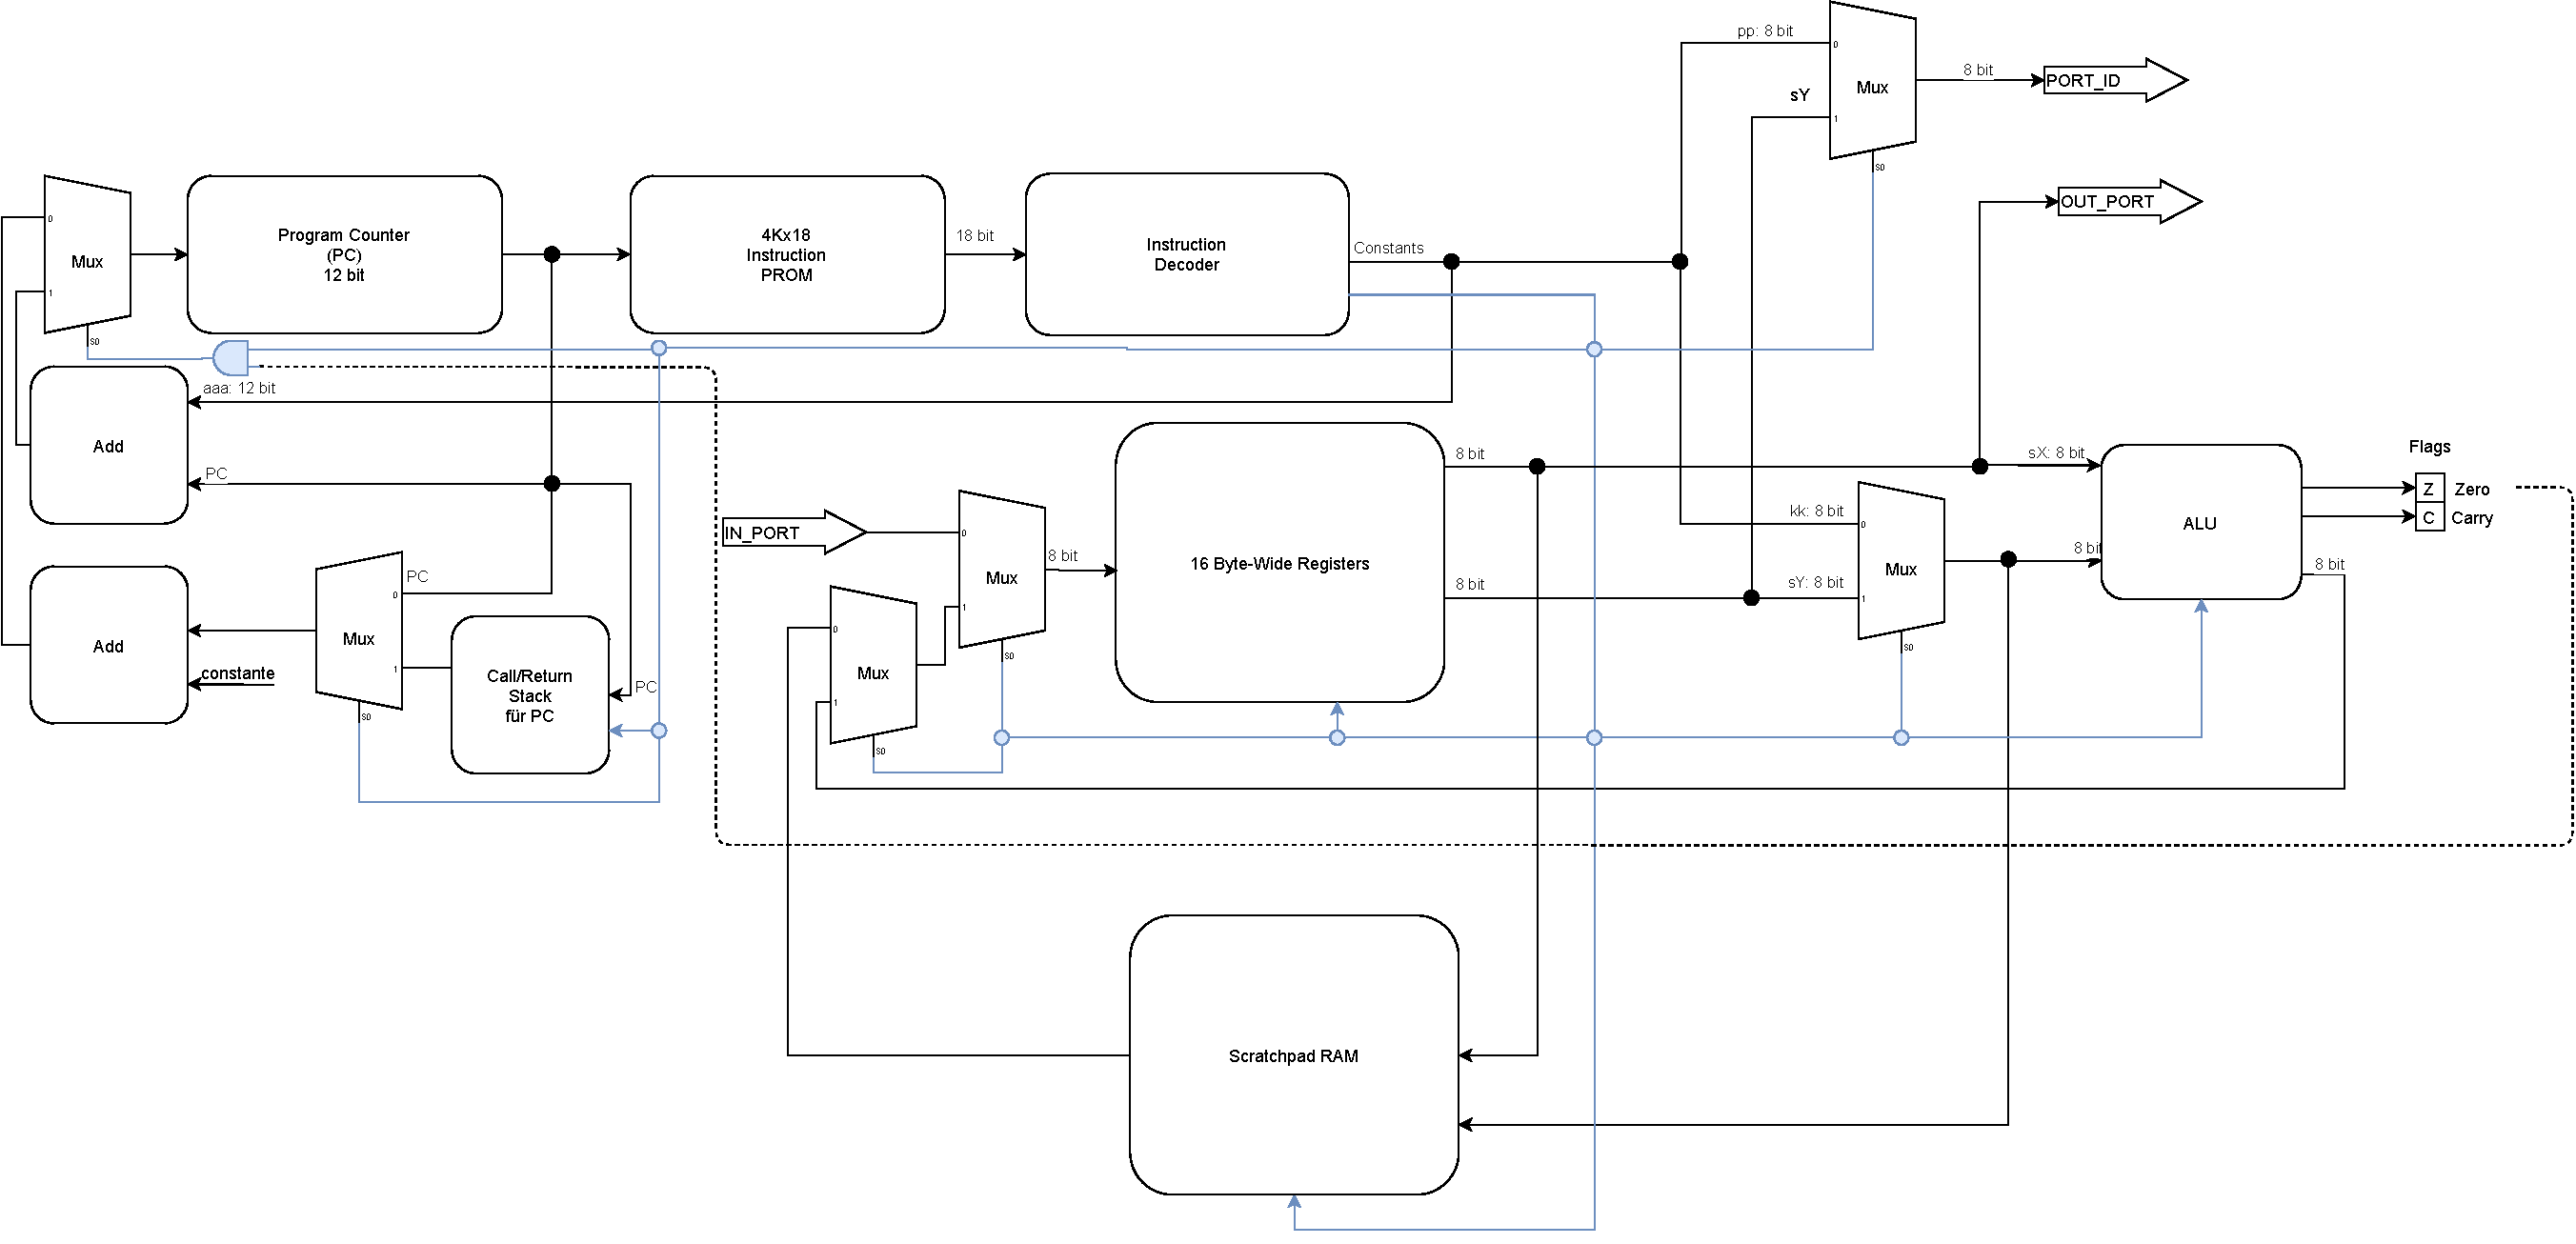
\includegraphics[width=\textwidth, angle=0]{Blockdiagram.pdf}


\section{Blockbeschreibungen}
\subsection{ALU}
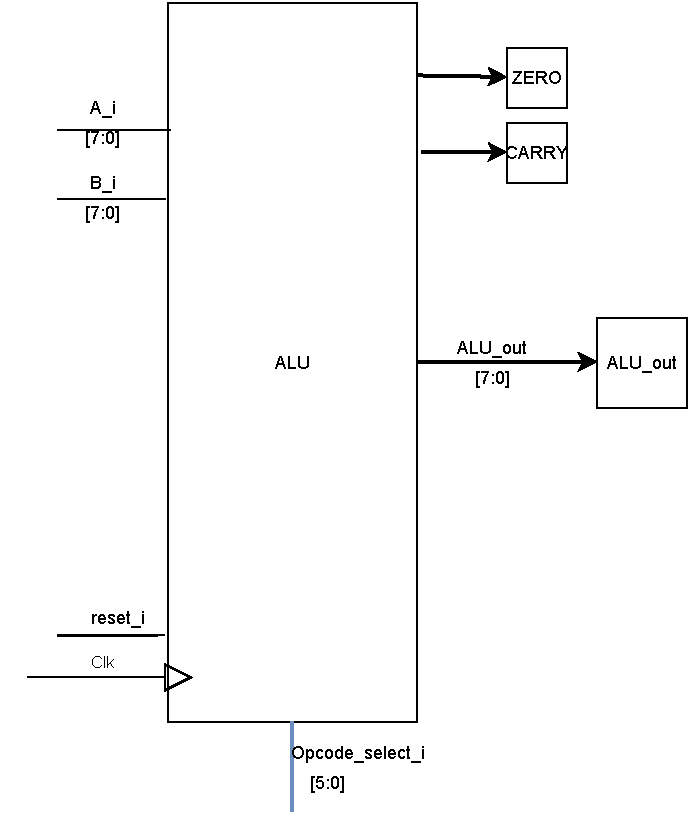
\includegraphics[height=0.6\textheight, angle=0]{ALU_beschreibung.pdf}\\
Die ALU führt Operationen auf zwei Eingabedaten aus. Die Operationen umfassen Arithmetische, Logische Verknüpfungen und Shift Operationen. Die Eingabedaten sind entweder Konstante Werte vom Instruction Decoder (kk) oder aus den Registern (sX,sY) geladene Werte. Sie werden an den Eingängen sA\_i und sB\_i angelegt. Der opcode\_select\_i Eingang (vom Instruction Decoder), entscheidet darüber, welche Operation auf den Eingabedaten ausgeführt wird. Das Ergebnis der ausgeführten Operation wird an sALU\_o angelegt.
Die sZERO\_o und sCARRY\_o ausgänge werden je nach Operation, entsprechend der unten aufgeführten Tabelle, gesetzt.
\subsection{Instruction Decoder}
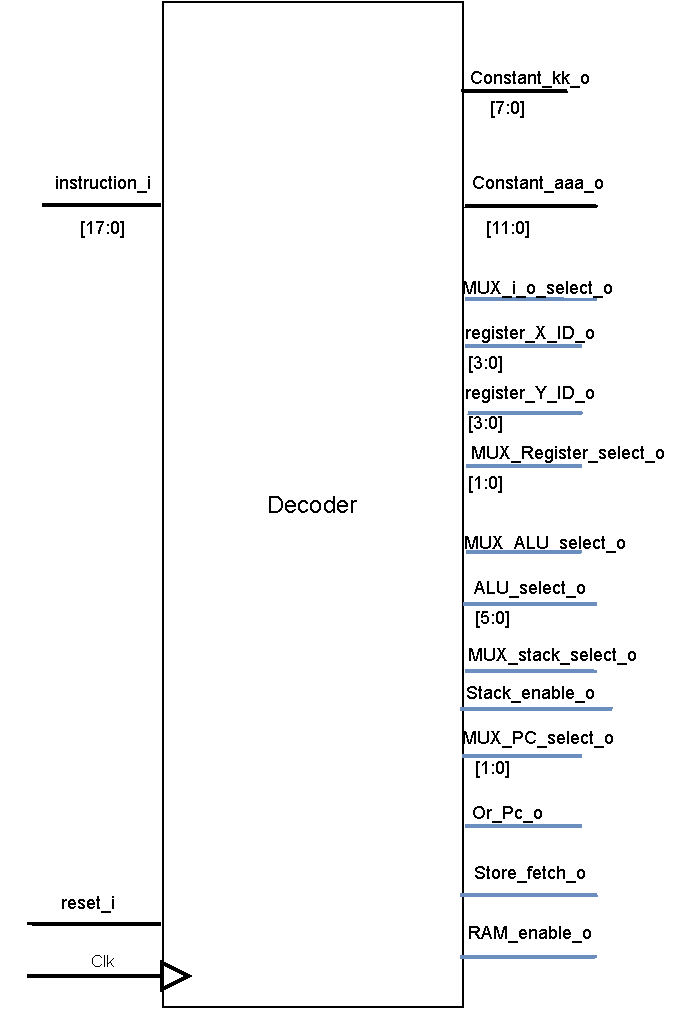
\includegraphics[height=0.7\textheight, angle=0]{ID_beschreibung.pdf}\\
Der Instruction Decoder (ID) dekodiert die aus dem Instruktionsspeicher geladenen Befehle und sendet entsprechende Steuersignale an die einzelnen Komponenten. Die Instruktionen, die vom ID verarbeitet werden, liegen am Eingang instruction\_i in form von 18 bit an. Je nach Instruktion, werden die Werte an den Ausgänge des ID entsprechend gesetzt. An sRegister\_X\_adresse\_o und sRegister\_Y\_adresse\_o werden die in den Instruktionen vorhandenen Register Adressen ausgegeben und ans Register weitergeleitet.
Enthält die Instruktion konstanten, so werden diese entsprechen an die Ausgänge constant\_kk\_o (8 bit) und const\_aaa\_o (12 bit) angelegt. Die mux\_... Ausgänge, sowie der or\_PC\_o Ausgang, leiten entsprechend der eingegangenen Instruktion Steuerbits an verschiedene Multiplexer weiter. Der sALU\_select\_o Ausgang gibt den Opcode der Instruction an die ALU weiter. Der sRam\_write\_or\_read\_o Ausgang signalisiert dem Speicher, ob ein Wert gelesen oder geschrieben werden soll. Die sRegister\_write\_enable\_o , sStack\_enable\_o, sRAM\_write\_or\_read\_o und sRAM\_enable\_o Ausgänge, steuern den zugriff auf Register, Stack und RAM.
\subsection{Program Counter}
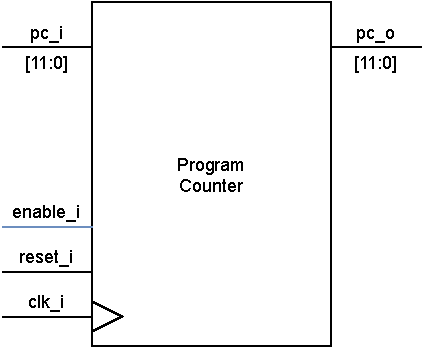
\includegraphics[]{ProgramCounter_beschreibung (2).pdf}\\
Der Program Counter zeigt mit den Outputbits pc\_o auf die Position im Instruktionsspeicher, an welcher der aktuelle Befehl steht, der in den Instruktions Decoder geladen werden soll um ausgeführt zu werden. Bei jeder rising edge am clk\_i Input werden, falls das enable\_i Bit auf 1 gesetzt ist, die momentanen pc\_i Bits auf die pc\_o Bits übertragen, und damit der nächste Befehl geladen. \\
Durch ein setzten des reset\_i Bits auf 1 kann der Program Counter asynchron auf den ersten Befehl zurückgesetzt werden.
\subsection{scratchpad RAM}
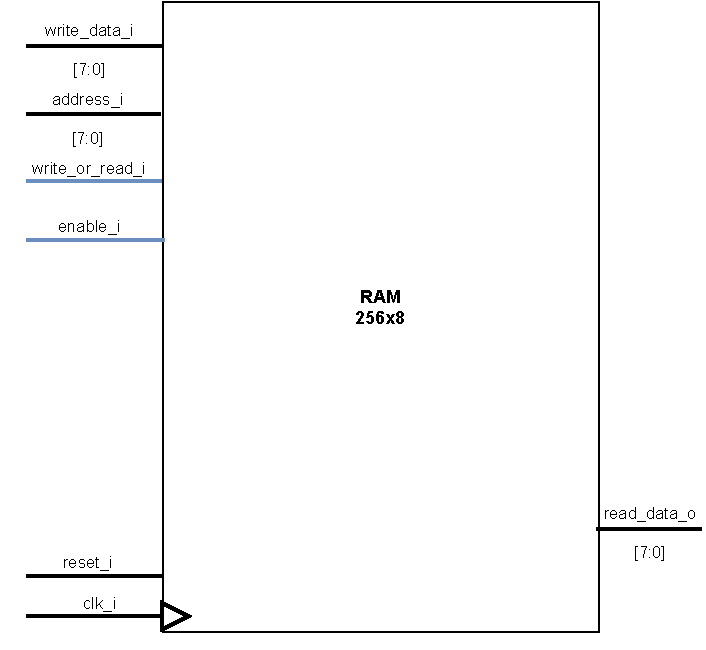
\includegraphics[]{RAM_beschreibung.pdf}\\
Ein Zusätzlicher Speicher um Werte zu Speichern. Das write\_or\_read bit bestimmt ob gelesen oder geschreiben wird. Es wird entweder von address\_i auf read\_data gelesen  oder es wird write\_data auf address\_i geschrieben. address\_i kommt entweder aus dem Register oder vom Instruction decoder. write\_data und read\_data sind beide mit dem Register verbunden. Es wird nur in den RAM geschrieben wenn enable auf 1 gesetzt ist.
\subsection{Register}
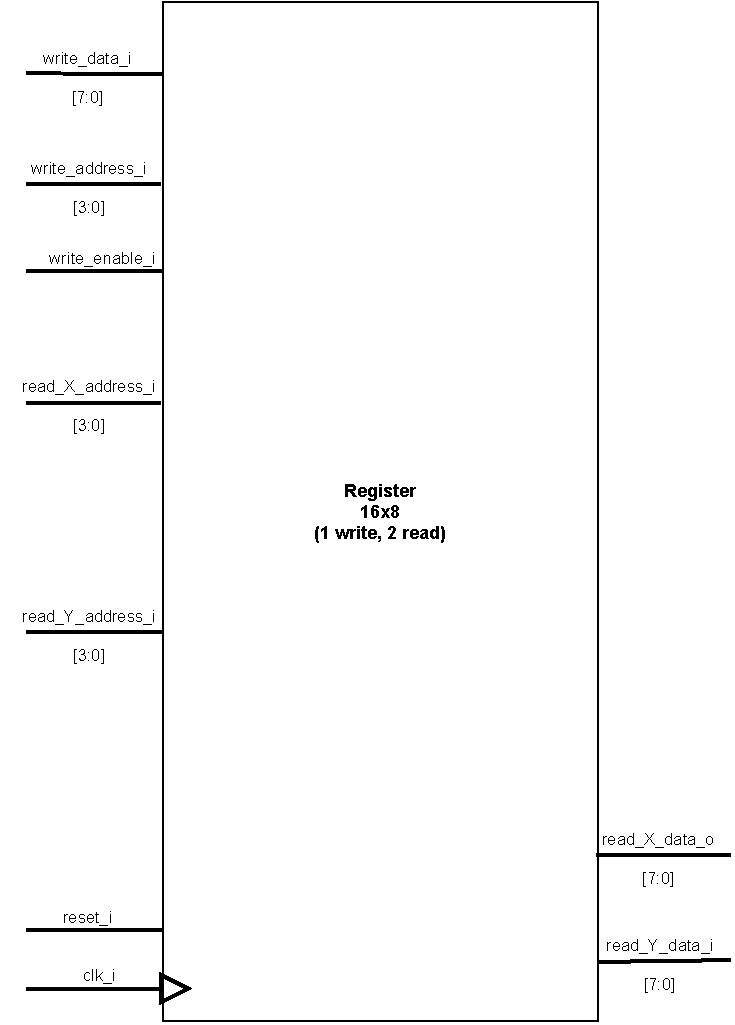
\includegraphics[]{Register_beschreibung.pdf}\\
Speichert 8bit Werte. Ergebnisse der ALU werden meist hierhin geschrieben. Das Register hat einen 8-bit breiten Eingang write\_data\_i um Daten anzunehmen, welche gespeichert werden sollen. Hierzu gibt es noch einen 4-bit breiten Eingang write\_address\_i um das Register auszuwählen und das write\_enable\_i bit um das schreiben zu aktivieren. Um aus dem Register zu lesen gibt es zwei Eingänge read\_X\_address\_i und read\_Y\_address\_i um die Register auszuwählen und zwei Ausgänge read\_X\_data\_o read\_Y\_data\_o auf welchen die Daten ausgegeben werden. So können zwei Werte aus dem Register gelesen werden. Über den reset\_i Eingang lässt sich das gesamte Register auf 0-Einträge zurücksetzen.
\subsection{Instruction Memory}
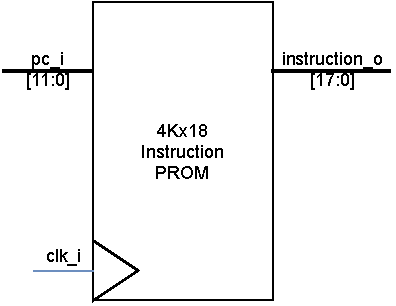
\includegraphics[height=0.4\textheight, angle=0]{IP_beschreibung.pdf}\\
Ein Speicher in dem die Instruktionen als 18 Bit Werte gespeichert werden. Der Input(pc\_i) beschreibt die Stelle im Speicher, die derzeit ausgeführt wird und deshalb am Ausgang instruction\_o für den Instruction Decoder bereitliegt. Ändert sich der Input pc\_i ändert sich der Ausgang instruction\_o mit der nächsten steigenden Taktflanke von clk\_i.
\subsection{CALL/RETURN Stack}
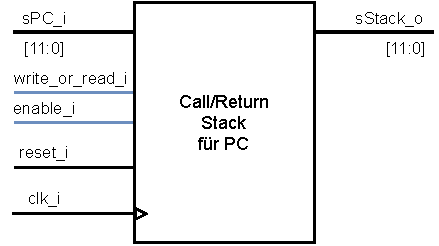
\includegraphics[width=0.7\textwidth, angle=0]{Stack_beschreibung.pdf}\\
Ein Stackspeicher, der die Position des Program Counters vor einem Unterfunktionsaufruf speichert. Dabei werden die bei sPC\_i anliegenden Bits auf den Stack gespeichert, wenn write\_or\_read\_i auf 0 gesetzt ist, enable\_i auf 1 gesetzt ist und bei clk\_i ein rising edge vorliegt. Ist dagegen write\_or\_read\_i auf 1, werden bei der nächsten rising edge von clk\_i die oben auf dem Stack liegenden Bits auf den sStack\_o Output übertragen und vom Stack gelöscht. Ist enable\_i auf 0, so werden weder Daten auf den Stack gelegt, noch welche von ihm genommen. \\
Durch ein setzten von reset\_i auf 1 lässt sich der Stack asynchron resetten und damit leeren.

\subsection{Input/Output}
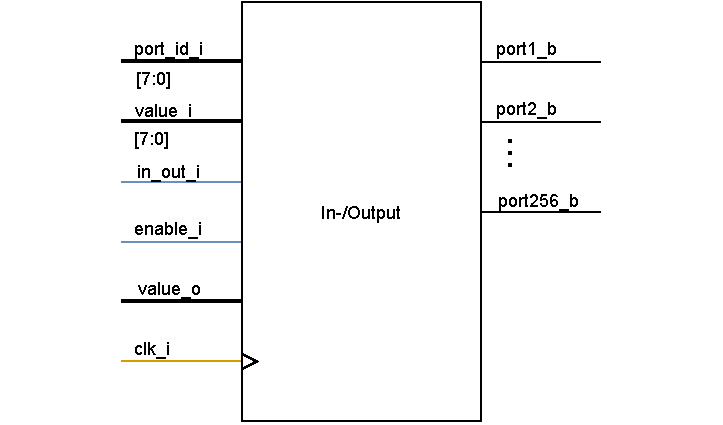
\includegraphics[height=0.5\textheight, angle=0]{IO_beschreibung.pdf}\\
Die nach außen zu sendenden Signale(erhalten durch value\_i) werden am Port mit der Nummer gegeben durch port\_id\_i ausgegeben, falls in\_out\_i und enable\_i den Wert 1 enthält. Falls enable\_i den Wert 1 und in\_out\_i 0 enthält, wird der derzeit anliegende Wert beim Port der port\_id\_i in value\_o gespeichert.
\newpage
\section{Instruktionen}


%\begin{table}[h!]
    %\centering
    \begin{longtable}{||c|p{4cm}|c||}
        \hline \hline
         Instruktion & Beschreibung & Funktion  \endhead \hline
         ADD sX, kk & Addiert zum Register sX das Literal kk hinzu. & sX $\leftarrow$ sX + kk  \\ \hline
         ADD sX, sY & Addiert zum Register sX den Inhalt aus Register sY hinzu. & sX $\leftarrow$ sX + sY   \\ \hline
         ADDCY sX, kk & Addiert zum Register sX das Literal kk mit Carry-Bit hinzu. &sX $\leftarrow$ sX+kk+CARRY   \\ \hline
         ADDCY sX, sY & Addiert zum Register sX den Inhalt aus Register sY mit Carry-Bit hinzu. & sX $\leftarrow$ sX+sY+CARRY  \\ \hline
         AND sX, kk & Bitweises UND von Register sX mit dem Literal kk. & sX $\leftarrow$ sX AND kk  \\ \hline
         AND sX, sY & Bitweises UND von Register sX mit Register sY. & sX $\leftarrow$ sX AND sY  \\ \hline
          CALL aaa & Bedingungsloser Aufruf der Unterfunktion an der Adresse aaa. &TOS $\leftarrow$ PC, PC $\leftarrow$ aaa  \\ \hline
         CALLC aaa & Falls CARRY-Bit gesetzt, Aufruf der Unterfunktion an der Adresse aaa. &if CARRY =1 {TOS $\leftarrow$ PC, PC $\leftarrow$ aaa}  \\ \hline
         CALLNC aaa & Falls CARRY-Bit nicht gesetzt, Aufruf der Unterfunktion an der Adresse aaa. &if CARRY =0 {TOS $\leftarrow$ PC, PC $\leftarrow$ aaa} \\ \hline
         CALLNZ aaa & Falls ZERO-Bit nicht gesetzt, Aufruf der Unterfunktion an der Adresse aaa. &if ZERO=0 {TOS $\leftarrow$ PC, PC $\leftarrow$ aaa}  \\ \hline
         CALLZ aaa & Falls ZERO-Bit gesetzt, Aufruf der Unterfunktion an der Adresse aaa. &if ZERO=1{TOS $\leftarrow$ PC, PC $\leftarrow$ aaa}\\ \hline
         COMPARE sX, kk & Vergleicht Register sX mit dem Literal kk. Setzt das CARRY und ZERO flag wie angegeben, Register bleiben dabei unverändert. & \makecell{if sX = kk ZERO $\leftarrow$ 1, \\ if sX \textless $ $ kk CARRY $\leftarrow$ 1 }  \\ \hline
         COMPARE sX, sY & Vergleicht Register sX mit dem Register sY. Setzt das CARRY und ZERO flag wie angegeben, Register bleiben dabei unverändert. & \makecell{sX = sY ZERO $\leftarrow$ 1, \\ if sX \textless $ $ sY CARRY $\leftarrow$ 1  }  \\ \hline
         FETCH sX, (sY) & Lese scratchpad RAM von der in Register sY gespeicherten Adresse in Register sX &sX $\leftarrow$ RAM[(sY)]   \\ \hline
         FETCH sX, ss & Lese scretchpad RAM von Adresse ss in Register sX &sX $\leftarrow$ RAM[ss]  \\ \hline
         INPUT sX, (sY) & Lese Wert des Input-Port, welcher vom Register sY spezifiziert wird, in das Register sX. &PORT\_ID $\leftarrow$ sY, sX $\leftarrow$ IN\_PORT  \\ \hline
         INPUT sX, pp & Lese Wert des Input-Port, welcher von pp spezifiziert wird, in das Register sX. &PORT\_ID $\leftarrow$ pp, sX $\leftarrow$ IN\_PORT \\ \hline
         JUMP aaa & Bedingungsloser Sprung nach aaa. &pc $\leftarrow$ aaa  \\ \hline
         JUMPC aaa & Falls das CARRY-Bit gesetzt ist, springe zu aaa. & if CARRY=1 pc $\leftarrow$ aaa \\ \hline
         JUMPNC aaa & Falls das CARRY-Bit nicht gesetzt ist, springe zu aaa. &if CARRY=0 pc $\leftarrow$ aaa  \\ \hline
         JUMPNZ aaa & Falls das ZERO-Bit nicht gesetzt ist, springe zu aaa. &if ZERO=0 pc $\leftarrow$ aaa  \\ \hline
         JUMPZ aaa & Falls das ZERO-Bit gesetzt ist, springe zu aaa. &if ZERO=1 pc $\leftarrow$ aaa  \\ \hline 
         LOAD sX, kk & Lade das Literal kk in das Register sX. &sX $\leftarrow$ kk   \\ \hline
         LOAD sX, sY & Lade den Inhalt des Registers sY in das Register sX. &sX $\leftarrow$ sX  \\ \hline 
         OR sX, kk & Bitweise OR von Register sX mit literal kk. &sX $\leftarrow$ sX OR kk   \\ \hline
         OR sX, sY & Bitweise OR von Register sX mit Register sY. & sX $\leftarrow$ sX OR sY   \\ \hline
         OUTPUT sX, (sY) & Schreibe Register sX zum in sY gespeicherten output Port. &PORT\_ID $\leftarrow$ sY, OUT\_PORT $\leftarrow$ sX  \\ \hline
         OUTPUT sX, pp & Schreibe Register sX zu output Port pp. &PORT\_ID $\leftarrow$ pp, OUT\_PORT $\leftarrow$ sX  \\ \hline
         RETURN & Bedingungslose Rückkehr von der Unterfunktion. & PC $\leftarrow$ TOS+1  \\ \hline
         RETURNC & Falls Carry-Bit gesetzt, Rückkehr von der Unterfunktion. & If CARRY=1, PC $\leftarrow$ TOS+1 \\ \hline
         RETURNNC & Falls Carry-Bit nicht gesetzt, Rückkehr von der Unterfunktion. & If CARRY=0, PC $\leftarrow$ TOS+1 \\ \hline
         RETURNZ & Falls Zero-Bit gesetzt, Rückkehr von der Unterfunktion.& If ZERO=1, PC $\leftarrow$ TOS+1 \\ \hline
         RETURNNZ & Falls Zero-Bit nicht gesetzt, Rückkehr von der Unterfunktion. & If ZERO=0, PC $\leftarrow$ TOS+1  \\ \hline
         RL sX & Rotiert Register sX einen Schritt nach links. &sX $\leftarrow$ {sX[6:0],sX[7]}, CARRY $\leftarrow$ sX[7]  \\ \hline
         RR sX & Rotiert Register sX einen Schritt nach rechts. &sX $\leftarrow$ {sX[0],sX[7:1]},CARRY $\leftarrow$ sX[0]   \\ \hline
         SL0 sX & Schiebe Register sX links, mit 0 aufgefüllt. &sX $\leftarrow$ {sX[6:1],0}, CARRY $\leftarrow$ sX[7]  \\ \hline
         SL1 sX & Schiebe Register sX links, mit 1 aufgefüllt. &sX $\leftarrow$ {sX[6:1],1}, CARRY $\leftarrow$ sX[7]  \\ \hline
         SLA sX & Schiebe Register sX links durch alle Bits, inklusive Carry. &sX $\leftarrow$ {sX[6:1],CARRY}, CARRY $\Leftarrow$ sX[7]  \\ \hline
         SLX sX & Schiebe Register sX links. Bit sX[0] unbetroffen. &sX $\leftarrow$ {sX[6:1],sX[0]}, CARRY $\leftarrow$ sX[7]  \\ \hline
         SR0 sX & Schiebe Register sX rechts, mit 0 aufgefüllt. &sX $\leftarrow$ {0,sX[7:1]}, CARRY $\leftarrow$ sX[0]  \\ \hline
         SR1 sX & Schiebe Register sX rechts, mit 1 aufgefüllt. &sX $\leftarrow$ {1,sX[7:1]}, CARRY $\leftarrow$ sX[0]  \\ \hline
         SRA sX & Schiebe Register sX durch alle bits, inklusive Carry. &sX $\leftarrow$ {CARRY,sX[7:1]}, CARRY $\leftarrow$ sX[0]  \\ \hline
         SRX sX & Arithmetisches rechtsschieben von Register sX mit Vorzeichenerweiterung. &sX $\leftarrow$ {s[7],sX[7:1]}, CARRY $\leftarrow$ sX[0]  \\ \hline
         STORE sX, (sY) & Schreibe Register sX in scratchpad RAM an der in Register sY gespeicherten Adresse. &RAM[(sY)] $\leftarrow$ sX \\ \hline
         STORE sX, ss & Schreibe Register sX an Adresse ss in scratchpad RAM. &RAM[ss] $\leftarrow$ sX \\ \hline
         SUB sX, kk & Subtrahiere literal kk von Register sX. &sX $\leftarrow$ sX-kk  \\ \hline
         SUB sX, sY & Subtrahiere Register sY von Register sX. &sX $\leftarrow$ sX-sY  \\ \hline
         SUBCY sX, kk & Subtrahiere literal kk von Register sX mit Carry. &sX $\leftarrow$ sX-kk-CARRY  \\ \hline
         SUBCY sX, sY & Subtrahiere Register sY von Register sX mit Carry. &sX $\leftarrow$ sX-sY-CARRY  \\ \hline
         TEST sX, kk & Teste Bits in Register sX gegen literal kk. Update Carry und Zero flags. Register bleiben unverändert. & \makecell{if(sX AND kk)=0 ZERO $\leftarrow$ 1, \\ CARRY $\leftarrow$ odd parity of (sX AND kk) }   \\ \hline
         TEST sX, sY  & Teste Bits in Register sX gegen Bits in Register sY. Update Carry und Zero flags. Register bleiben unverändert. & \makecell{if(sX AND sY)=0 ZERO $\leftarrow$ 1, \\ CARRY $\leftarrow$ odd parity of (sX AND sY) }  \\ \hline
         XOR sX, kk & Bitweise XOR von Register sX mit literal kk. &sX $\leftarrow$ sX XOR kk  \\ \hline
         XOR sX, sY & Bitweise XOR von Register sX mit Register sY. &sX $\leftarrow$ sX XOR sY   \\ \hline
         
    \end{longtable}
    %\caption{Caption}
    %\label{tab:my_label}
%\end{table}

\newpage
\begin{longtable}{||c|p{6cm}|p{6cm}|c||}
\hline \hline
    Instruktion & ZERO & CARRY & opcode   \endhead \hline
    ADD sX, kk & if (sX + kk = (0 or 256)): ZERO = 1,\newline else: ZERO = 0
    & if ((sX + kk) $>$ 255): CARRY = 1,\newline else: CARRY = 0 & 000001 \\ \hline
    ADD sX, sY & if (sX + sY = (0 or 256)): ZERO = 1,\newline else: ZERO = 0
    & if ((sX + sY) $>$ 255): CARRY = 1,\newline else: CARRY = 0 & 000000 \\ \hline
    ADDCY sX, kk & if (sX + kk + CARRY = (0 or 256)): ZERO = 1,\newline else: ZERO = 0
    & if ((sX + kk + CARRY) $>$ 255): CARRY = 1,\newline else: CARRY = 0 & 000011 \\ \hline
    ADDCY sX, sY & if (sX + sY + CARRY = (0 or 256)): ZERO = 1,\newline else: ZERO = 0
    & if ((sX + sY + CARRY) $>$ 255): CARRY = 1,\newline else: CARRY = 0 & 000010 \\ \hline
    AND sX, kk & if (sX = 0): ZERO = 1,\newline else: ZERO = 0 & 0 & 001001 \\ \hline
    AND sX, sY & if (sX = 0): ZERO = 1,\newline else: ZERO = 0 & 0 & 001000 \\ \hline
    CALL aaa & - & - & 100001 \\ \hline
    CALLC aaa  & - & - & 100010 \\ \hline
    CALLNC aaa & - & - & 100011 \\ \hline
    CALLNZ aaa & - & - & 100100 \\ \hline
    CALLZ aaa & - & - & 100101 \\ \hline
    COMPARE sX, kk & if (sX = kk): ZERO = 1,\newline else: ZERO = 0
    & if (kk $>$ sX): CARRY = 1,\newline else: CARRY = 0 & 011011 \\ \hline
    COMPARE sX, sY & if (sX = sY): ZERO = 1,\newline else: ZERO = 0
    & if (sY $>$ sX): CARRY = 1,\newline else: CARRY = 0 & 011010 \\ \hline
    FETCH sX, (sY) & - & - & 010010 \\ \hline
    FETCH sX, ss & - & - & 010011 \\ \hline
    INPUT sX, (sY) & - & - & 010110 \\ \hline
    INPUT sX, pp & - & - & 010111 \\ \hline
    JUMP aaa & - & - & 100110 \\ \hline
    JUMPC aaa & - & - & 100111 \\ \hline
    JUMPNC aaa & - & - & 101000 \\ \hline
    JUMPNZ aaa & - & - & 101001 \\ \hline
    JUMPZ aaa & - & - & 101010 \\ \hline 
    LOAD sX, kk & - & - & 001111 \\ \hline
    LOAD sX, sY & - & - & 001110 \\ \hline 
    OR sX, kk & if (sX = 0): ZERO = 1,\newline else: ZERO = 0 & 0 & 001011 \\ \hline
    OR sX, sY & if (sX = 0): ZERO = 1,\newline else: ZERO = 0 & 0 & 001010 \\ \hline
    OUTPUT sX, (sY) & - & - & 010100 \\ \hline
    OUTPUT sX, pp & - & - & 010101 \\ \hline
    RETURN & - & - & 111010 \\ \hline
    RETURNC & - & - & 111011 \\ \hline
    RETURNNC & - & - & 111100 \\ \hline
    RETURNZ & - & - & 111101 \\ \hline
    RETURNNZ & - & - & 111110 \\ \hline
    RL sX & if (sX = 0): ZERO = 1,\newline else: ZERO = 0
    & CARRY = sX[7] & 110000 \\ \hline
    RR sX & if (sX = 0): ZERO = 1,\newline else: ZERO = 0
    & CARRY = sX[0] & 110001 \\ \hline
    SL0 sX & if (sX = 0): ZERO = 1,\newline else: ZERO = 0
    & CARRY = sX[7] & 110010 \\ \hline
    SL1 sX & if (sX = 0): ZERO = 1,\newline else: ZERO = 0
    & CARRY = sX[7] & 110011 \\ \hline
    SLA sX & if (sX = 0): ZERO = 1,\newline else: ZERO = 0
    & CARRY = sX[7] & 110100 \\ \hline
    SLX sX & if (sX = 0): ZERO = 1,\newline else: ZERO = 0
    & CARRY = sX[7] & 110101 \\ \hline
    SR0 sX & if (sX = 0): ZERO = 1,\newline else: ZERO = 0
    & CARRY = sX[0] & 110111 \\ \hline
    SR1 sX & if (sX = 0): ZERO = 1,\newline else: ZERO = 0
    & CARRY = sX[0] & 110111 \\ \hline
    SRA sX & if (sX = 0): ZERO = 1,\newline else: ZERO = 0
    & CARRY = sX[0] & 111000 \\ \hline
    SRX sX & if (sX = 0): ZERO = 1,\newline else: ZERO = 0
    & CARRY = sX[0] & 111001 \\ \hline
    STORE sX, (sY) & - & - & 010000 \\ \hline
    STORE sX, ss & - & - & 010001 \\ \hline
    SUB sX, kk & if ((sX - kk) = 0): ZERO = 1,\newline else: ZERO = 0
    & if ((sX - kk) $<$ 0): CARRY = 1,\newline else: CARRY = 0 & 000101 \\ \hline
    SUB sX, sY & if ((sX - sY) = 0): ZERO = 1,\newline else: ZERO = 0
    & if ((sX - sY) $<$ 0): CARRY = 1,\newline else: CARRY = 0 & 000100 \\ \hline
    SUBCY sX, kk & if ((sX - kk- CARRY) = (0 or -256): ZERO = 1,\newline else: ZERO = 0
    & if ((sX - kk - CARRY) $<$ 0): CARRY = 1,\newline else: CARRY = 0 & 000111 \\ \hline
    SUBCY sX, sY & if ((sX - sY - CARRY) = (0 or -256): ZERO = 1,\newline else: ZERO = 0
    & if ((sX - sY - CARRY) $<$ 0): CARRY = 1,\newline else: CARRY = 0 & 000110 \\ \hline
    TEST sX, kk & if (AND\textunderscore TEST = 0): ZERO = 1,\newline else: ZERO = 0
    & if (XOR\textunderscore TEST = 1): CARRY = 1,\newline else: CARRY = 0 & 011001 \\ \hline
    TEST sX, sY  & if (AND\textunderscore TEST = 0): ZERO = 1,\newline else: ZERO = 0
    & if (XOR\textunderscore TEST = 1): CARRY = 1,\newline else: CARRY = 0 & 011000 \\ \hline
    XOR sX, kk & if (sX = 0): ZERO = 1,\newline else: ZERO = 0 & 0 & 001101 \\ \hline
    XOR sX, sY & if (sX = 0): ZERO = 1,\newline else: ZERO = 0 & 0 & 001100 \\ \hline
\end{longtable}

\newpage
\section{Aufgabenaufteilung}

    \begin{longtable}{||c|c|c|c|c|c|c|c|c||}
        \hline \hline
         Nr. & Arbeitspaket & JG & TW & JB & AB & OAK & SN & JU \endhead \hline
         10 & Instruktionen & * &  &  & * &  &  &\\ \hline
         20 & Blockdiagram &  &  & * &  &  & * & \\ \hline
         30 & Register &  & * &  &  &  &  &\\ \hline
         40 & RAM & * &  &  &  &  &  &\\ \hline
         50 & PC &  &  &  &  &  & & * \\ \hline
         51 & Instruction Memory &  &  & *  &  &  & &  \\ \hline
         60 & I/O &  &  & *  &  &  & &  \\ \hline
         71 & ALU Aritmetik &  &  &  &  & * &  & \\ \hline
         72 & ALU Logik &  &  &  &  &  & * & \\ \hline
         73 & ALU Shift &  &  &  & * &  &  & \\ \hline
         74 & \makecell{ALU Verifikation \\ 10 einfache Testfälle }&  &  &  &  &  & * & \\ \hline
         80 & Decoder &  &  &  &  & * &  & \\ \hline
         90 & Assembler &  &  &  & * &  &  & \\ \hline
         100 & Test Register &  &  & * &  &  &  &\\ \hline
         110 & Test RAM &  &  &  &  &  &  & *\\ \hline
         120 & Test PC &  &  &  &  &  & * &  \\ \hline
         130 & Test I/O &  &  &  & * &  & &  \\ \hline
         140 & Test ALU & * &  &  &  &  &  & \\ \hline
         150 & Test Decoder &  & * &  &  &  &  & \\ \hline
    \end{longtable}


\end{document}
